\chapter{Evaluation}
\label{Evaluation}

In order to evaluate the quality of the \aicat\ framework, several
aspects of the framework have been tested.  The three main areas
tested are quality of categorization, efficiency, and ease of use.
For testing the quality of categorization and efficiency, performance
is measured on categorization tasks using several different data sets.

Section \ref{Corpora} describes the data sets used during testing.
Section \ref{Quality} presents various measurements of how accurately
the framework performs on these data sets, and Section
\ref{Efficiency} discusses the computational efficiency of the
framework.  Section \ref{Applications} discusses the ease of use of
the framework in different contexts.


\section{Corpora}
\label{Corpora}

During development and testing, several data sets, or ``corpora,''
were used for framework testing and application building.  Since the
framework will behave differently on different data sets, it is
important to understand the characteristics of each corpus.  For
instance, different feature selection and categorization algorithms
may scale differently in relation to the size of the training corpus,
both in terms of efficiency and accuracy. \cite{chakrabarti:98} Also,
the specifics of the categorization problem in each corpus may be more
amenable to one categorization technique or another.

The corpora used for evaluation are listed in this section.  Each
corpus consists of a set of documents $\docs$, a set of categories $\cats$ that
documents may be assigned to, and a domain-expert-made choice of
category assignments for each document.  These category assignments
are considered to be completely correct, and they form a standard
against which the TC system's categorization on the test documents can
be measured.  For each corpus, the set $\docs$ is divided into a
training set $\train$ and a test set $\test$.

Unless otherwise noted below, a list of common English words from
\cite{salton:89} was used as a ``stoplist,'' or a set of terms to
completely ignore when processing documents.  This is a common technique from
Information Retrieval \cite[sec. 15.1.1]{manning:99}, as it is assumed that these words
possess little or no information about the target categories, and that
they will only slow processing and add noise to the data.


\subsection{ApteMod}


The ApteMod version of the Reuters-21578 corpus has become a standard
benchmark corpus in evaluating Text Categorization
systems. \cite{yang:99,joachims:98} In terms of evaluating the \aicat\
framework, it provides an opportunity to compare the performance of
\aicat\ with other implementations of the same TC algorithms so that
the correctness of the present implementation can be verified.

ApteMod is a collection of 10,788 documents from the Reuters financial
newswire service, partitioned into a training set with 7769
documents and a test set with 3019 documents.  The total size of the
corpus is about 43 MB.  It is available for download from
\url{http://kdd.ics.uci.edu/databases/reuters21578/reuters21578.html}.

The distribution of categories in the ApteMod corpus is highly skewed,
with 36.7\% of the documents in the most common category, and only
0.0185\% (2 documents) in each of the five least common categories.
In fact, the original data source is even more skewed---in creating
the corpus, any categories that did not contain at least one document
in the training set and one document in the test set were removed from
the corpus. \cite{yang:99}

In the ApteMod corpus, each document belongs to one or more
categories.  There are 90 categories in the corpus.  The average
number of categories per document is 1.235, and the average number of
documents per category is about 148, or 1.37\% of the corpus.

\begin{figure}
\begin{center}
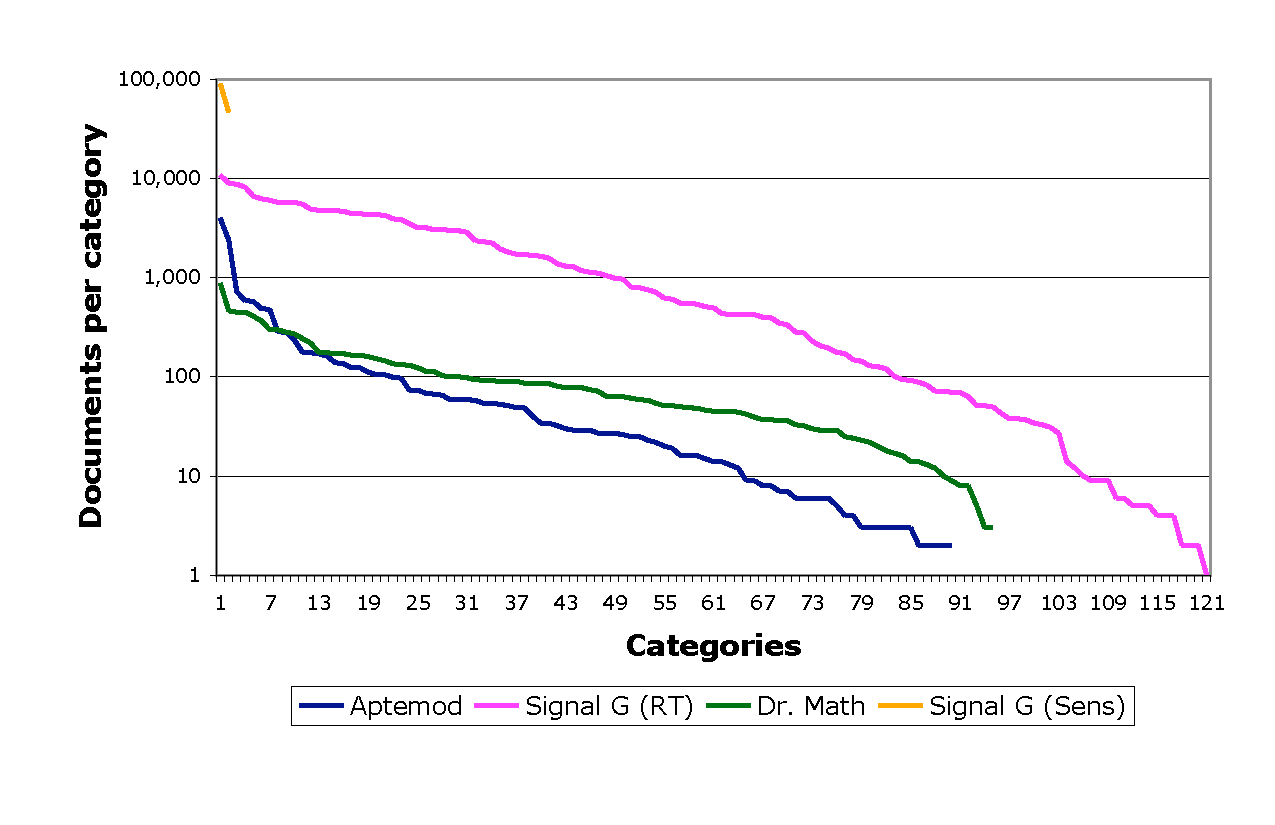
\includegraphics[width=\linewidth]{figures/Corpora-catdist.pdf}
\caption{Category distributions for the test corpora}
\label{Corpora-catdist}
\end{center}
\end{figure}

Figure \ref{Corpora-catdist} shows the category distribution for
the corpora discussed in this section.  The categories are plotted on
the horizontal axis, and the number of documents per category are
plotted on the vertical axis using a logarithmic scale.


\subsection{Dr. Math}

The ``Ask Dr. Math'' service \cite{drmath} is one of many so-called
ask-an-expert services becoming common on the Internet.  These
services are generally staffed by domain experts who answer questions
about the domain sent by non-experts.  Ask-an-expert services may be
chiefly educational, as the Ask Dr. Math service is, or they may be
tied to businesses' Customer Relationship Management or support
initiatives.

Since the domain experts in these services often have a single
subdomain of expertise, it is helpful if they can view only the subset
of the questions that relate to that subdomain.  However, the
non-experts may not know how to properly categorize their own question
when submitting it.  For example, a user of the Ask Dr. Math service
may be a middle school student unfamiliar with the particular
mathematics taxonomy used by the service.  It may therefore be
infeasible for the users to categorize questions during submission,
and it is in this situation that automatic categorization may be
helpful.

The Dr. Math corpus is a collection of 6,630 English-language messages
sent to the ``Ask Dr. Math'' ask-an-expert service for
students. \cite{drmath} Each message has been manually assigned by a
domain expert to one or more categories,
with category names indicating both math topic and grade level,
e.g. ``High School Geometry.''  There are 95 categories in the
category set.  The ontology is generally not
separable into two separate category sets for independent topic and
level categorizations, in part because many topic and level
combinations like ``Elementary School Calculus'' don't exist in the
category scheme.

The 26 MB corpus is divided into a training set with 5,304 documents
and a test set with 1,326 documents.  As with the ApteMod corpus, the
category distribution is skewed, with 13.2\% of the documents in the
most common category and only 0.0452\% (3 documents) in the least
common category.  The average number of categories per document is
1.534, and the average number of documents per category is about 107,
or 1.61\% of the corpus.

The Dr. Math corpus is an important data set for proving the
effectiveness of the \aicat\ framework, because it represents a
potential real-world application in the educational domain, one of the key
target application areas of the Web Engineering Group at the
University of Sydney. Work with the Dr. Math corpus has been
previously published in \cite{williams:03}.

The Dr. Math corpus is not available for direct download, but interested
parties may contact the author for details.


\section{Quality of Categorization}
\label{Quality}

In order to evaluate the quality of the results generated by the
\aicat\ implementation code, categorization experiments were performed
on each of the corpora described in Section \ref{Corpora} using the
measures defined in Sections \ref{measures} and
\ref{combining-measures}.

Several
experimental parameters (e.g. category membership thresholds) can be
set for each experiment; for the ApteMod corpus these were set to
match the parameters used in \cite{yang:99}, where known.  For the
other corpora they were optimized to provide the
best performance on the test set---in this sense, the test set might
be thought of more correctly as a validation set, because in a strict
testing environment the performance on the test set should not
influence training parameters.  This methodology was adopted because
it more closely matches the procedure that would be used when building
an application, in which the true test set may consist of documents
not yet possessed by the developer, i.e. the set of target documents
in the application domain.  This is the evaluation method used in
several studies in the literature, such as \cite{joachims:98}.

Where a baseline score is given in the results, this refers to a
simple probabilistic categorizer that assigns categories to each
document, weighting the probability of assignment by the frequency of
each category in the training set.  For instance, if a certain
category was present in 40\% of the training documents, any document
in the test set would have a probability of 0.4 of being assigned to
that category by the baseline categorizer.  

It should be emphasized that this thesis does not claim to produce any
new results in the area of developing Text Categorization algorithms.
Descriptions of existing algorithms from the TC literature have formed
the basis for developing the \aicat\ framework.  The results presented
here should be considered successful if they align with results
already published in the literature---superior results should not be
expected.

\subsection{ApteMod}

Table \ref{aptemod-results} summarizes the results of three different
machine learning methods in \aicat\ as compared with the baseline
categorizer described above.  Table \ref{aptemod-yang} gives similar
scores from a well-known comparative study of common categorization
algorithms. \cite{yang:99} Where possible, the present study has
attempted to duplicate the findings in \cite{yang:99}, though in some
cases there is not enough information to duplicate the findings
exactly, and in some cases the \aicat\ framework lacks certain
features mentioned in \cite{yang:99}.  These differences will be
discussed below.

\begin{table}
\begin{center}
\begin{tabular}{|r c c c c c c c|}
\hline
%              maR       maP       maF1      miR          miP         miF1
method    & $\rho^M$ & $\pi^M$ & $F_1^M$ & $\rho^\mu$ & $\pi^\mu$ & $F_1^\mu$ &   error \\
\hline
NB        &   .3659  &  .4969  &  .3959  &  .7238     &  .8514    &  .7824    &  .00555 \\
SVM       &   .0868  &  .3727  &  .1239  &  .5254     &  .9106    &  .6663    &  .00725 \\
kNN       &   .2655  &  .3856  &  .2903  &  .7650     &  .7975    &  .7809    &  .00591 \\
Baseline  &   .0135  &  .0142  &  .0137  &  .1645     &  .1664    &  .1654    &  .02287 \\
\hline
\end{tabular}
\end{center}
\caption{Results of \aicat\ on ApteMod corpus}
\label{aptemod-results}
\end{table}

\begin{table}
\begin{center}
\begin{tabular}{|r c c c c c c c|}
\hline
method & $\rho^M$ & $\pi^M$ & $F_1^M$ & $\rho^\mu$ & $\pi^\mu$ & $F_1^\mu$ & error \\
\hline
NB  & - & - & .3886 & .7688 & .8245 & .7956 & .00544 \\
SVM & - & - & .5251 & .8120 & .9137 & .8599 & .00365 \\
kNN & - & - & .5242 & .8339 & .8807 & .8567 & .00385 \\
\hline
\end{tabular}
\end{center}
\caption{Results from \cite{yang:99} on ApteMod corpus}
\label{aptemod-yang}
\end{table}

In the case of the \naive\ Bayes categorizer (NB), the results match
\cite{yang:99} closely, with a slightly greater $F_1^M$ and a slightly
smaller $F_1^\mu$.  To match the experimental
settings in \cite{yang:99}, the size of the feature-set was set to
2000.

For the Support Vector Machine categorizer (SVM), the performance is
significantly worse than the findings in \cite{yang:99}.  The reasons
for this are not clear---\aicat\ currently uses an SVM implementation
based on the \texttt{libsvm} C library \cite{libsvm}, whereas
\cite{yang:99} used $SVM^{light}$ as its
implementation\cite{joachims:99a}, and there may be major differences
in the behavior of these two libraries.  Since the macro-averaged scores are
particularly bad, it may be inferred that \cite{libsvm} is not
performing well on rare categories.  In both studies, a linear SVM
kernel was used, and 10,000 features were considered when building the
categorization model.

One possible reason for the poor performance of the SVM categorizer is
that for both micro- and macro-averaged scores, $\pi$ is much larger
than $\rho$, indicating that this situation could be balanced by
choosing more appropriate category membership thresholds.  However,
\texttt{libsvm} doesn't seem to allow tuning of these thresholds, so a
remedy for this situation isn't clear.

For the k-Nearest-Neighbor categorizer (kNN), $F_1^\mu$ results are comparable
with NB, but no scores are as good as the kNN results in \cite{yang:99}.
The major difference between the two implementations is that the
implementation in \cite{yang:99} finds per-category membership
thresholds by optimizing performance on a validation set, while the
implementation in \aicat\ uses a single membership threshold for all
categories, settable by the user.  In this experiment the threshold
was set to 0.1, a value which is not meaningful in itself, but which
seemed to give the best performance.  Note, that the macro-averaged
precision is higher than recall, but the micro-averaged recall is
higher than precision, indicating that it is not possible to
simultaneously find the optimal threshold for both rare and common
categories.  Thus using individual thresholds for each category should
increase $F_1$ scores if optimized properly.  The $k$ parameter
in this experiment
(indicating the number of similar documents to consider when
categorizing) was set to 45, and the number of features considered was
set to 2415, both to match the values used in \cite{yang:99}.

The kNN implementation in \aicat\ is fairly new, and is an adaptation
of work by another researcher.  The ability to optimize per-category
thresholds is considered a useful future addition to the framework,
and will be added soon.

For all three categorizers, the \param{tfidf\_weighting} parameter was set to
\texttt{xfx}, indicating that words are weighted by the logarithm of
their inverse document frequency.  This is the same setting used in
\cite{yang:99}.  One other possible difference between \cite{yang:99}
and the current experiment is that \cite{yang:99} used either a
$\chi^2$ or \emph{information gain} criterion (it is not clear which
criterion was used with which categorizer) for feature selection,
while \emph{document frequency} was used here.  This should not be a
major factor in the results, as document frequency has been shown to
produce results competitive with other feature selection methods on
this corpus. \cite{yang:97}



\subsection{Dr. Math}

Table \ref{drmath-results} shows the categorization performance of
\aicat\ on the Dr. Math corpus.  Note that the baseline micro-averaged
scores are much lower than on the ApteMod corpus (Table
\ref{aptemod-results}), indicating that this may be a more difficult
categorization task simply because the category distribution is
flatter than in ApteMod (Figure \ref{Corpora-catdist}).


\begin{table}
\begin{center}
\begin{tabular}{|r c c c c c c c|}
\hline
%              maR       maP       maF1      miR          miP         miF1
method    & $\rho^M$ & $\pi^M$ & $F_1^M$ & $\rho^\mu$ & $\pi^\mu$ & $F_1^\mu$ &   error \\
\hline
NB        &   .2338  &  .2677  &  .2358  &  .3766     &  .3542    &  .3651    &  .0215  \\
SVM       &   .3333  &  .1562  &  .1946  &  .4211     &  .2273    &  .2952    &  .0330  \\
kNN       &   .2372  &  .2824  &  .2154  &  .3607     &  .3572    &  .3590    &  .0212  \\
Baseline  &   .0156  &  .0176  &  .0161  &  .0406     &  .0421    &  .0413    &  .0310  \\
\hline
\end{tabular}
\end{center}
\caption{Results of \aicat\ on Dr. Math corpus}
\label{drmath-results}
\end{table}

Because no other TC study has been done on the Dr. Math corpus, not
much can be said about the comparative results of the \aicat\
framework.  However, the noteworthy points will be discussed below.

Using the \naive\ Bayes categorizer, the $F_1$ scores are about 0.24
when macro-averaged and 0.37 when micro-averaged.  This is not as
dramatic a difference as seen on the ApteMod corpus, where the
micro-averaged scores are approximately double the macro-averaged
scores.  In this experiment, the number of features considered was set
to 20\% of the training corpus, or 1764 features, though varying this
parameter between 1500 and 3000 seemed to produce similar results.

Using the SVM categorizer, $F_1$ scores were again worse than with NB,
but in this case the recall with SVM was higher than the
precision---the opposite of the situation on the ApteMod corpus.
Again, a mechanism for trading off $\rho$ and $\pi$ would be
desirable.  The best scores with SVM were obtained when using no
feature selection at all, i.e. using all 8824 features when building
the SVM models.  This is an indication of SVM's robustness to noise in
the data sets it considers.

With the kNN categorizer, results were competitive with the NB
categorizer.  Note that $F_1^M$ for kNN is lower than each of $\rho^M$
and $\pi^M$---this somewhat counterintuitive situation, unique to
macro-averaging, can arise when the per-category scores $\rho_i$ are
sometimes greater than $\pi_i$ and sometimes less than $\pi_i$.  The
best results for this experiment were found when using a feature set
with 3000 features and $k=15$.


\section{Efficiency}
\label{Efficiency}

In order to assess the efficiency of the implementations in \aicat,
the running times and memory usage of the framework on the tasks in
Section \ref{Quality} are reported here.  All tests were performed on
a Sun Ultra-Enterprise server running Solaris 7, with a processor
speed of 400 MHz, and with 2040 Megabytes of RAM.  The software used
was a pre-release version of \aicat\ version 0.05, running under perl
version 5.6.1.

The reader is cautioned that the resource usage numbers presented here
will be highly volatile from one system to another, and that they may
even change significantly with different versions of the software
running on the same system.  The results presented here may give a
rough indication of how the efficiency of different techniques relate
to each other, however, and how the sizes of the data sets affect
efficiency.

Each experiment is divided into four stages, each run as a separate
system process:

\begin{description}
\item[Scan] The training corpus $\train$ is scanned to determine the
  most relevant features, using the document frequency feature
  selection criterion, and the list of relevant features is saved to
  disk.
\item[Read] The entire training corpus $\train$ is read into memory as
  a \class{KnowledgeSet}, using only the features determined in the
  ``Scan'' step, and saved to disk as a data structure accessible for the
  next step.
\item[Learn] A \class{Learner} object is created, and its
  \method{train} method is invoked using the \class{KnowledgeSet} from
  the previous step.  The \class{Learner} is saved for use in the next
  step.
\item[Test] The \class{Learner} from the previous step is loaded into
  memory, and each document from the test corpus $\test$ is
  categorized using the \class{Learner}'s \method{categorize} method.
\end{description}

\begin{table}
\begin{center}
\begin{tabular}{|c|r|r r r r|}
\cline{3-6}
\multicolumn{2}{c|}{}
                 &  Scan  &  Read   &  Learn  &  Test   \\ \hline
           & NB  & 128.6s & 122.8s  &   22.9s &  244.2s \\
ApteMod    & SVM & 133.1s & 126.6s  & 2332.3s &  448.2s \\
           & kNN & 126.9s & 121.8s  &   21.5s & 2616.2s \\ \hline
           & NB  &  44.8s &  43.2s  &    7.2s &   46.7s \\
Dr. Math   & SVM &  43.7s &  42.8s  &  734.5s &  118.9s \\
           & kNN &  43.8s &  42.2s  &    6.6s &  725.2s \\ \hline
\end{tabular}
\end{center}
\caption[Time required for the experiments in Section \ref{Quality}]
 {Time required for the experiments in Section \ref{Quality}.
  Measurements are given in CPU seconds.}
\label{eval-time}
\end{table}

\begin{table}
\begin{center}
\begin{tabular}{|c|r|r r r r|}
\cline{3-6}
\multicolumn{2}{c|}{}
                 &  Scan &  Read  & Learn  & Test  \\ \hline
           & NB  & 10.5M & 48.7M  & 47.0M  & 13.6M \\
ApteMod    & SVM & 12.2M & 50.6M  & 876.6M & 31.1M \\
           & kNN & 10.8M & 48.0M  & 64.4M  & 44.1M \\ \hline
           & NB  & 8.7M  & 24.1M  & 24.1M  & 11.0M \\
Dr. Math   & SVM & 9.4M  & 26.3M  & 304.7M & 21.5M \\
           & kNN & 9.0M  & 25.1M  & 28.1M  & 21.9M \\ \hline
\end{tabular}
\end{center}
\caption[Memory usage for the experiments in Section \ref{Quality}]
 {Memory usage for the experiments in Section \ref{Quality}.
  Measurements are given in megabytes of virtual memory usage.}
\label{eval-memory}
\end{table}

Table \ref{eval-time} shows the running times for each phase of the
experiments conducted in Section \ref{Quality}, and Table
\ref{eval-memory} shows their memory usage.
Running time is given in total CPU seconds consumed,
and memory usage is measured by reporting the total size of the
process in virtual memory.\footnote{On Unix operating systems,
  including the Solaris system on which these tests were performed,
  the term ``virtual memory'' when describing the size of a process
  means the total size of the running process, including any memory
  segments in Random Access Memory and any cached to the disk.  It
  does not refer just to the portion that may be resident on the disk
  cache, as the term is sometimes used to mean on Windows or older
  Macintosh systems.}
Note that the running times include both
the loading of any data structures from the previous stage and the
saving of any data structures for the next stage.  The memory usage
includes any data structures used by the application as well as the
perl interpreter itself.

Of course, the running times and memory usage during the ``Scan'' and
``Read'' stages do not vary much when the Machine Learning algorithm
is changed, because this part of the process does not involve the
\class{Learner} class.  The numbers are presented so that the reader
may compare the measurements on the different corpora, and any
unexpected differences are likely due to the state of other concurrent
processes on the machine, caching of disk data, and the like.

Among the most obvious characteristics of the results in Tables
\ref{eval-time} and \ref{eval-memory} is that the \naive\ Bayes
categorizer is very efficient in terms of both running time and
memory.  The SVM categorizer is slower during the ``Learn'' phase by a
factor of about 100, and the kNN categorizer is slower during the
``Test'' phase by a factor of 10--20.  This is consistent with the
theoretical properties of the algorithms discussed in Section
\ref{machine-learning}.

One other interesting property is that the SVM categorizer seems to
take roughly twice as much time and memory as the NB categorizer
during the ``Test'' phase.  This is not necessarily supported by the
theoretical properties of the two algorithms, so this finding may be
due to implementation issues in the SVM code or the Adapter to the SVM
engine.


\section{Applications}
\label{Applications}

Unfortunately, there are as yet no standard methods of objectively
evaluating the quality of a framework's design.  Such a method is not
likely to appear in the near future, because framework design is a
highly subjective process requiring much expertise in the framework
developer. \cite[sec. 1.5]{fayad:99} Some quality metrics have been
proposed, but they tend to rely on comparing different releases of a
framework as it evolves to meet application needs, interpreting any
major changes as flaws in the original framework
design. \cite[ch. 25]{fayad:99} Because \aicat\ is a newly released
framework, this kind of comparison between releases is not possible.

In order to provide evidence of the framework's usefulness, therefore,
one option is simply to build different kinds of applications using
the framework and judge whether the applications were successful or
not, and whether the framework seemed well-suited for the application.
Ideally, the applications will represent at least some of the use
cases that the framework was designed to support.  This is what will
be done here.  Three applications using \aicat\ that were developed
during the course of the candidature on which this thesis is based
will be discussed in the following sections.

\subsection{Command-line categorizer}

The first framework is a simple command-line script, distributed with
the framework code, which provides a relatively simple way to
instantiate a top-level \aicat\ object and invoke several of its
methods.  Its main purpose is to support the kinds of scientific
investigations described in Section \ref{scientific-inv}.

Using this script, the user may specify the parameters for an
experiment either directly on the command line, or in a file of
key-value pairs indicating the parameter's name and value.  A sample
file of this sort is shown in Figure \ref{parameter-file}.

\begin{figure}
\begin{code}
--- #YAML:1.0
data_root: corpora/drmath-1.00
stopword_file: corpora/drmath-1.00/SMART.stoplist
progress_file: "/tmp/drmath-NB"
outfile: "results/drmath-NB.txt"
learner_class: "::NaiveBayes"
tfidf_weighting: xfx
stemming: porter
features_kept: 0.2
verbose: 1
\end{code}
\caption{Parameter specification file for testing the \naive\ Bayes
  categorizer on the Dr. Math corpus.}
\label{parameter-file}
\end{figure}

This command-line application also provides support for storing the
sets of parameters and the categorization results to disk.  In this
way, the user keeps a historical record of which parameter settings
improved performance and which had negative effects.

This application contains only 110 lines of Perl code, most of which
deals with benchmarking issues or parsing of the command-line
options.  This shows that a data-driven application can be built on
top of the framework fairly easily.

\subsection{Database categorization}

In order to support the categorization of documents inside a database
as mentioned in Sections \ref{embedded-apps} and \ref{database}, David
Bell of the Web Engineering Group at the University of Sydney
developed an application which embeds \aicat\ directly in the
PostgreSQL database engine.  Bell's work involved the kNN categorizer,
but because the framework was used instead of a custom kNN
implementation, any of the framework's categorizers could be used in
the same manner.

Using this application, categorization functionality was made
available in database insertions and queries through the use of
embedded functions like \method{categorize}.  This allows
categorization of arbitrary text in the database, because the input to
the categorization function is any string that can be built using the
database query language.

This application demonstrates the ability of the \aicat\ framework to
provide functionality in embedded environments.

\subsection{Client-server categorization}

As part of a research project in the financial domain, Mark Aufflick
of the Web Engineering Group at the University of Sydney created a
categorization server like that described in Section
\ref{client-server}.  In this application, the categorizer resides in
a long-lived server daemon process that accepts XML/RPC requests for
categorizing arbitrary documents.  The server responds with the
categorization information as an XML/RPC response, which may contain
the categories assigned or the single best category assigned.

The application was built using standard Perl tools for constructing
XML\discretionary{/}{}{/}RPC servers, available from the CPAN.  This demonstrates the
ability of the \aicat\ framework to build custom categorization
servers for diverse application needs.
